\documentclass{standalone}
\usepackage{tikz}
\usetikzlibrary{patterns, positioning}
\usepackage[sfdefault]{ClearSans} %% option 'sfdefault' activates Clear Sans as the default text font
\usepackage[T1]{fontenc}

\begin{document}
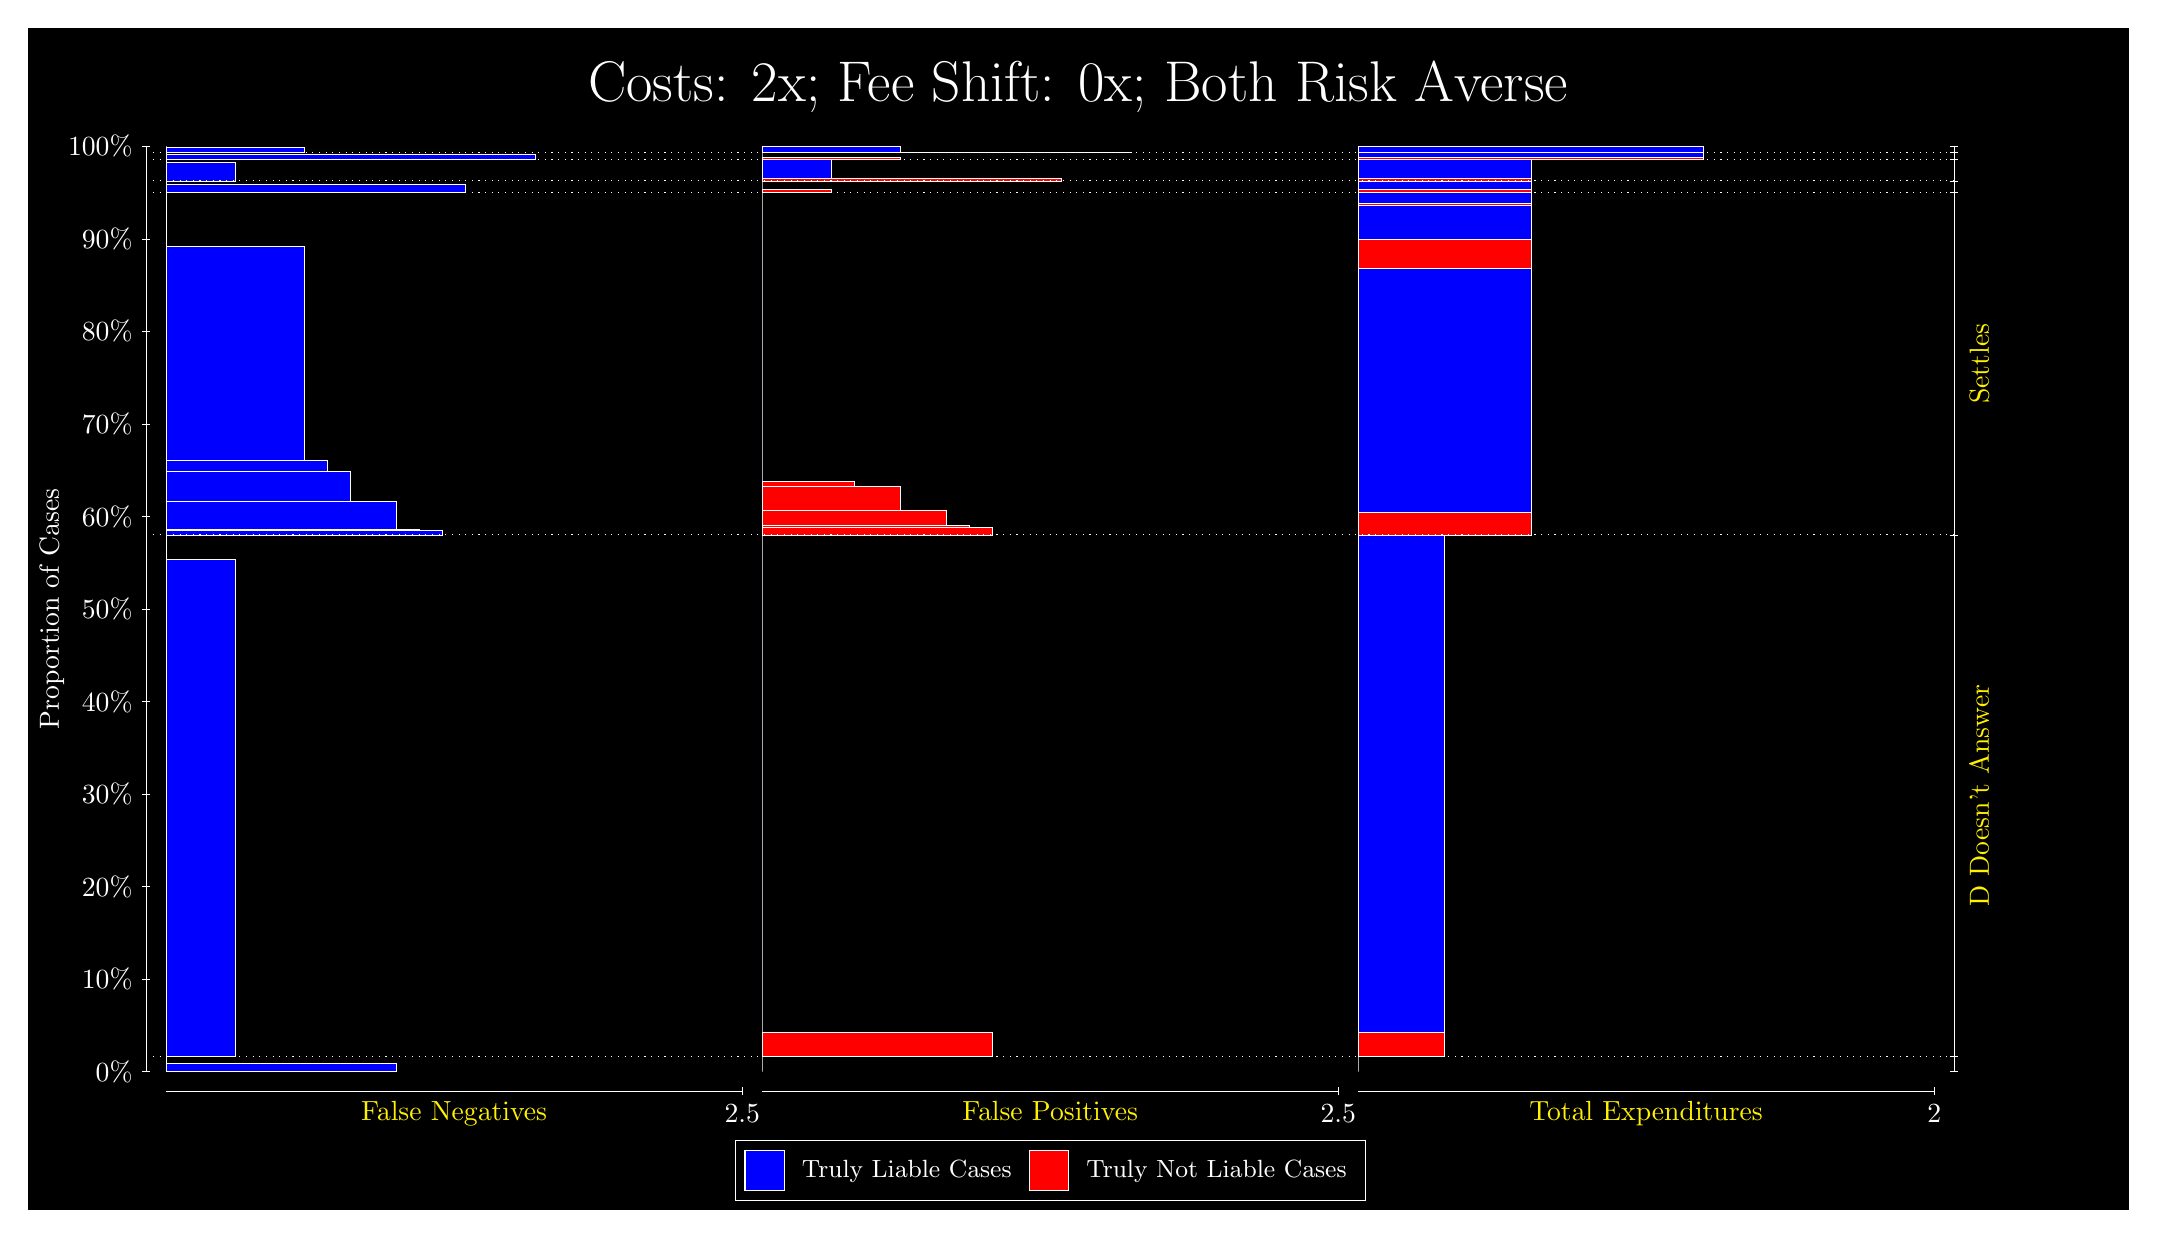
\begin{tikzpicture}
\draw[fill=black] (0,0) rectangle (26.667,15);
\draw[text=white] (0,13.5) rectangle (26.667,15) node[midway] {\huge Costs: 2x; Fee Shift: 0x; Both Risk Averse};
\draw[white, very thin] (1.5,1.75) -- (1.5,13.5);
\node[rotate=90, text=white, anchor=center] at (0.3, 7.625) {Proportion of Cases};
\draw[white, very thin] (1.45,1.75) -- (1.55,1.75);
\node[text=white, anchor=east] at (1.45, 1.75) {0\%};
\draw[white, very thin] (1.45,2.925) -- (1.55,2.925);
\node[text=white, anchor=east] at (1.45, 2.925) {10\%};
\draw[white, very thin] (1.45,4.1) -- (1.55,4.1);
\node[text=white, anchor=east] at (1.45, 4.1) {20\%};
\draw[white, very thin] (1.45,5.275) -- (1.55,5.275);
\node[text=white, anchor=east] at (1.45, 5.275) {30\%};
\draw[white, very thin] (1.45,6.45) -- (1.55,6.45);
\node[text=white, anchor=east] at (1.45, 6.45) {40\%};
\draw[white, very thin] (1.45,7.625) -- (1.55,7.625);
\node[text=white, anchor=east] at (1.45, 7.625) {50\%};
\draw[white, very thin] (1.45,8.8) -- (1.55,8.8);
\node[text=white, anchor=east] at (1.45, 8.8) {60\%};
\draw[white, very thin] (1.45,9.975) -- (1.55,9.975);
\node[text=white, anchor=east] at (1.45, 9.975) {70\%};
\draw[white, very thin] (1.45,11.15) -- (1.55,11.15);
\node[text=white, anchor=east] at (1.45, 11.15) {80\%};
\draw[white, very thin] (1.45,12.325) -- (1.55,12.325);
\node[text=white, anchor=east] at (1.45, 12.325) {90\%};
\draw[white, very thin] (1.45,13.5) -- (1.55,13.5);
\node[text=white, anchor=east] at (1.45, 13.5) {100\%};

\draw[white, very thin] (24.457,1.75) -- (24.457,13.5);
\draw[white, very thin] (24.407,1.75) -- (24.507,1.75);
\node[anchor=west] at (24.407, 1.75) {};
\draw[white, very thin] (24.407,1.942) -- (24.507,1.942);
\node[anchor=west] at (24.407, 1.942) {};
\draw[white, very thin] (24.407,8.5664) -- (24.507,8.5664);
\node[anchor=west] at (24.407, 8.5664) {};
\draw[white, very thin] (24.407,12.912) -- (24.507,12.912);
\node[anchor=west] at (24.407, 12.912) {};
\draw[white, very thin] (24.407,13.061) -- (24.507,13.061);
\node[anchor=west] at (24.407, 13.061) {};
\draw[white, very thin] (24.407,13.335) -- (24.507,13.335);
\node[anchor=west] at (24.407, 13.335) {};
\draw[white, very thin] (24.407,13.421) -- (24.507,13.421);
\node[anchor=west] at (24.407, 13.421) {};
\draw[white, very thin] (24.407,13.5) -- (24.507,13.5);
\node[anchor=west] at (24.407, 13.5) {};

\draw[white, very thin, fill=blue] (1.75,1.75) rectangle (4.6775,1.8586);
\draw[white, very thin, fill=red] (1.75,1.8586) rectangle (1.75,1.942);
\draw[white, very thin, fill=blue] (1.75,1.942) rectangle (2.6283,8.2589);
\draw[white, very thin, fill=red] (1.75,8.2589) rectangle (1.75,8.5664);
\draw[white, very thin, fill=blue] (1.75,8.5664) rectangle (5.2631,8.6268);
\draw[white, very thin, fill=blue] (1.75,8.6268) rectangle (4.9703,8.6306);
\draw[white, very thin, fill=blue] (1.75,8.6306) rectangle (4.6775,8.9951);
\draw[white, very thin, fill=blue] (1.75,8.9951) rectangle (4.092,9.3748);
\draw[white, very thin, fill=blue] (1.75,9.3748) rectangle (3.7993,9.5139);
\draw[white, very thin, fill=blue] (1.75,9.5139) rectangle (3.5065,12.236);
\draw[white, very thin, fill=red] (1.75,12.236) rectangle (1.75,12.912);
\draw[white, very thin, fill=blue] (1.75,12.912) rectangle (5.5558,13.016);
\draw[white, very thin, fill=red] (1.75,13.016) rectangle (1.75,13.061);
\draw[white, very thin, fill=blue] (1.75,13.061) rectangle (2.6283,13.303);
\draw[white, very thin, fill=red] (1.75,13.303) rectangle (1.75,13.335);
\draw[white, very thin, fill=blue] (1.75,13.335) rectangle (6.4341,13.397);
\draw[white, very thin, fill=red] (1.75,13.397) rectangle (1.75,13.421);
\draw[white, very thin, fill=blue] (1.75,13.421) rectangle (3.5065,13.493);
\draw[white, very thin, fill=red] (1.75,13.493) rectangle (1.75,13.5);
\draw[white, very thin, fill=red] (9.3189,1.75) rectangle (9.3189,1.8335);
\draw[white, very thin, fill=blue] (9.3189,1.8335) rectangle (9.3189,1.942);
\draw[white, very thin, fill=red] (9.3189,1.942) rectangle (12.246,2.2495);
\draw[white, very thin, fill=blue] (9.3189,2.2495) rectangle (9.3189,8.5664);
\draw[white, very thin, fill=red] (9.3189,8.5664) rectangle (12.246,8.6594);
\draw[white, very thin, fill=red] (9.3189,8.6594) rectangle (11.954,8.6841);
\draw[white, very thin, fill=red] (9.3189,8.6841) rectangle (11.661,8.8769);
\draw[white, very thin, fill=red] (9.3189,8.8769) rectangle (11.075,9.1842);
\draw[white, very thin, fill=red] (9.3189,9.1842) rectangle (10.783,9.1868);
\draw[white, very thin, fill=red] (9.3189,9.1868) rectangle (10.49,9.2433);
\draw[white, very thin, fill=blue] (9.3189,9.2433) rectangle (9.3189,12.912);
\draw[white, very thin, fill=red] (9.3189,12.912) rectangle (10.197,12.957);
\draw[white, very thin, fill=blue] (9.3189,12.957) rectangle (9.3189,13.061);
\draw[white, very thin, fill=red] (9.3189,13.061) rectangle (13.125,13.092);
\draw[white, very thin, fill=blue] (9.3189,13.092) rectangle (10.197,13.335);
\draw[white, very thin, fill=red] (9.3189,13.335) rectangle (11.075,13.359);
\draw[white, very thin, fill=blue] (9.3189,13.359) rectangle (9.3189,13.421);
\draw[white, very thin, fill=red] (9.3189,13.421) rectangle (14.003,13.428);
\draw[white, very thin, fill=blue] (9.3189,13.428) rectangle (11.075,13.5);
\draw[white, very thin, fill=red] (16.888,1.75) rectangle (16.888,1.8335);
\draw[white, very thin, fill=blue] (16.888,1.8335) rectangle (16.888,1.942);
\draw[white, very thin, fill=red] (16.888,1.942) rectangle (17.986,2.2495);
\draw[white, very thin, fill=blue] (16.888,2.2495) rectangle (17.986,8.5664);
\draw[white, very thin, fill=red] (16.888,8.5664) rectangle (19.083,8.8523);
\draw[white, very thin, fill=blue] (16.888,8.8523) rectangle (19.083,11.954);
\draw[white, very thin, fill=red] (16.888,11.954) rectangle (19.083,12.32);
\draw[white, very thin, fill=blue] (16.888,12.32) rectangle (19.083,12.749);
\draw[white, very thin, fill=red] (16.888,12.749) rectangle (19.083,12.773);
\draw[white, very thin, fill=blue] (16.888,12.773) rectangle (19.083,12.912);
\draw[white, very thin, fill=red] (16.888,12.912) rectangle (19.083,12.957);
\draw[white, very thin, fill=blue] (16.888,12.957) rectangle (19.083,13.061);
\draw[white, very thin, fill=red] (16.888,13.061) rectangle (19.083,13.092);
\draw[white, very thin, fill=blue] (16.888,13.092) rectangle (19.083,13.335);
\draw[white, very thin, fill=red] (16.888,13.335) rectangle (21.279,13.359);
\draw[white, very thin, fill=blue] (16.888,13.359) rectangle (21.279,13.421);
\draw[white, very thin, fill=red] (16.888,13.421) rectangle (21.279,13.428);
\draw[white, very thin, fill=blue] (16.888,13.428) rectangle (21.279,13.5);
\draw[white, dotted] (1.5,1.942) -- (24.457,1.942);
\draw[white, dotted] (1.5,8.5664) -- (24.457,8.5664);
\draw[white, dotted] (1.5,12.912) -- (24.457,12.912);
\draw[white, dotted] (1.5,13.061) -- (24.457,13.061);
\draw[white, dotted] (1.5,13.335) -- (24.457,13.335);
\draw[white, dotted] (1.5,13.421) -- (24.457,13.421);
\draw[white, very thin] (1.75,1.5) -- (9.0689,1.5);
\node[text=yellow, anchor=north] at (5.4094, 1.5) {False Negatives};
\draw[white, very thin] (9.0689,1.45) -- (9.0689,1.55);
\node[text=white, anchor=north] at (9.0689, 1.45) {2.5};

\draw[white, very thin] (9.3189,1.5) -- (16.638,1.5);
\node[text=yellow, anchor=north] at (12.978, 1.5) {False Positives};
\draw[white, very thin] (16.638,1.45) -- (16.638,1.55);
\node[text=white, anchor=north] at (16.638, 1.45) {2.5};

\draw[white, very thin] (16.888,1.5) -- (24.207,1.5);
\node[text=yellow, anchor=north] at (20.547, 1.5) {Total Expenditures};
\draw[white, very thin] (24.207,1.45) -- (24.207,1.55);
\node[text=white, anchor=north] at (24.207, 1.45) {2};


\node[text=yellow, centered, rotate=90] at (24.777, 5.2542) {D Doesn't Answer};
\node[text=yellow, centered, rotate=90] at (24.777, 10.739) {Settles};





\draw (12.978300999999998,1.5) node[draw=none] (baseCoordinate) {};
\begin{scope}[align=center]
        \matrix[scale=0.5, draw=white, below=0.5cm of baseCoordinate, nodes={draw}, column sep=0.1cm]{
            \node[rectangle, draw, minimum width=0.5cm, minimum height=0.5cm, fill=blue] {}; &
            \node[draw=none, font=\small, text=white] (B) {Truly Liable Cases}; &
            \node[rectangle, draw, minimum width=0.5cm, minimum height=0.5cm, fill=red] {}; &
            \node[draw=none, font=\small, text=white] (B) {Truly Not Liable Cases}; \\
            };
\end{scope}

\end{tikzpicture}
\end{document}